\chapter{Osciladores, números de ocupación y el primer campo cuántico}

La teoría cuántica de campos es el marco de prácticamente toda la física no gravitatoria conocida. Esta afirmación no debe confundirse con la idea de que se pueda resolver cualquier problema. El átomo de hidrógeno es manejable; al llegar a un átomo como el de boro, el cálculo ya es mucho más difícil, y un ser humano queda muy lejos de cualquier cálculo realista con teoría de campos. El marco puede ser fundamental aunque sus ecuaciones sigan siendo abrumadoramente difíciles.

Por tanto, nos adentraremos en el tema de la manera más elemental posible. A veces se lo llama \emph{segunda cuantización}, pero el nombre significará poco hasta que hayamos construido el formalismo. La ruta más corta no empieza con un campo relativista, sino con el oscilador armónico. Los resortes no son lo importante. Lo que importa es el álgebra de los operadores de creación y aniquilación. Cuando repitamos esa álgebra para muchos modos, un operador de creación dejará de significar simplemente ``elevar un oscilador un nivel'' y pasará a significar literalmente ``crear una partícula.''

\section{El oscilador como álgebra}

Para un oscilador, sea \(a^\dagger\) el operador que aumenta la excitación y sea \(a\) el que la disminuye. Las notaciones \(a_+\) y \(a_-\) son equivalentes, pero la notación con daga anticipa el lenguaje de la teoría de campos. El estado fundamental satisface
\begin{equation}
a|0\rangle=0,
\end{equation}
y el operador número es
\begin{equation}
N=a^\dagger a,
\qquad
N|n\rangle=n|n\rangle.
\end{equation}
Los dos operadores escalera son conjugados hermíticos, y su conmutador esencial es
\begin{equation}
[a,a^\dagger]=1.
\label{eq:l06-single-commutator}
\end{equation}
Esta pequeña álgebra es casi todo lo que hace falta del oscilador.

Se pueden obtener \(a\) y \(a^\dagger\) como combinaciones lineales adecuadas de la posición y el momento. La convención precisa depende de la normalización de \(x\), \(p\), \(m\) y \(\omega\); aquí, la afirmación útil e invariante es que \(a^\dagger a\) reconstruye el Hamiltoniano cuadrático del oscilador, salvo por la energía aditiva del estado fundamental. Así,
\begin{equation}
H=\hbar\omega\left(N+\frac12\right).
\end{equation}
Para lo que nos ocupa, omitimos el término constante y trabajamos con
\begin{equation}
H=\hbar\omega N.
\label{eq:l06-one-oscillator-hamiltonian}
\end{equation}
La frecuencia nos indica el coste de una excitación. Aumentar \(n\) en una unidad cuesta \(\hbar\omega\); disminuir \(n\) en una unidad libera esa misma cantidad.

\section{Muchos osciladores independientes}

Tomemos ahora muchos osciladores y etiquetémoslos con \(i\). Esta etiqueta es solo un índice, no la unidad imaginaria. Puede haber un número finito o infinito de modos. Una colección de resortes independientes ofrece una imagen; los modos normales de una cuerda de violín ideal ofrecen otra. En las aplicaciones a la teoría de campos, el caso importante es el de una colección infinita.

La independencia tiene un significado en términos de operadores. Los operadores que pertenecen a subsistemas verdaderamente independientes conmutan. Si no lo hicieran, las magnitudes correspondientes no podrían medirse independientemente y los sistemas no serían independientes de entrada. Por tanto, tenemos
\begin{align}
[a_i,a_j]&=0, \\
[a_i^\dagger,a_j^\dagger]&=0, \\
[a_i,a_j^\dagger]&=\delta_{ij}.
\label{eq:l06-many-commutators}
\end{align}
Para \(i\ne j\), todo lo que pertenece a los dos modos conmuta. Para \(i=j\), la última línea se reduce a la ecuación~\eqref{eq:l06-single-commutator}.

Cada oscilador tiene su propio operador número y, en general, su propia frecuencia:
\begin{equation}
N_i=a_i^\dagger a_i,
\qquad
H=\sum_i\hbar\omega_i N_i.
\label{eq:l06-many-hamiltonian}
\end{equation}
Un estado propio simultáneo queda etiquetado por la lista completa
\begin{equation}
|n_1,n_2,n_3,\ldots\rangle,
\qquad n_i=0,1,2,\ldots.
\label{eq:l06-occupation-ket}
\end{equation}
El entero \(n_i\) se llama \emph{número de ocupación} del oscilador \(i\). Por ahora, esto no es más que terminología. Pronto contará las partículas que ocupan un estado de una partícula, y el nombre adquirirá su sentido literal.

El estado en el que todos los números de ocupación son cero es
\begin{equation}
|0\rangle\equiv|0,0,0,\ldots\rangle,
\qquad a_i|0\rangle=0\quad\text{for every }i.
\label{eq:l06-oscillator-vacuum}
\end{equation}

\begin{classroomqa}
\lecturetimestamp{00:15:27}
\audiencequestion{¿Corresponde una familia infinita de osciladores al continuo de modos de un sistema como una cuerda de violín?}
\lecturerresponse{Sí, en el caso de la cuerda idealizada. Una cuerda real está hecha de átomos, así que, al llegar a longitudes de onda suficientemente cortas, aparece un límite microscópico. Aun así, el modelo continuo sirve de motivación para la colección infinita de modos que se usa en la teoría de campos.}
\end{classroomqa}

\section{Por qué los coeficientes de escalera son raíces cuadradas}

La acción de \(a^\dagger\) debe llevar un estado propio de \(N\) al siguiente estado propio, pero la normalización deja margen para un coeficiente:
\begin{equation}
a^\dagger|n\rangle=c_n|n+1\rangle.
\label{eq:l06-unknown-coefficient}
\end{equation}

\begin{figure}[htbp]
\centering
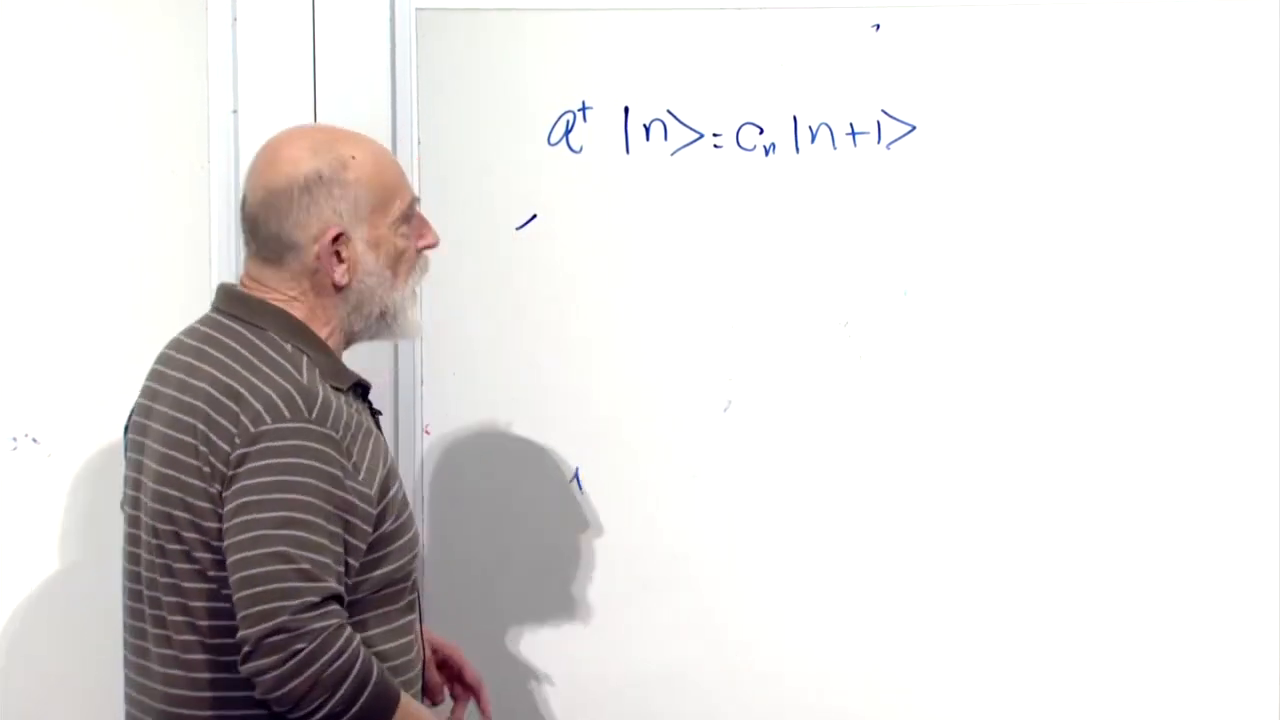
\includegraphics[width=0.9\linewidth]{lecture_06_frame_01.png}
\caption{El coeficiente de escalera se introduce antes de derivar su normalización. La ecuación de la pizarra se reproduce en la ecuación~\eqref{eq:l06-unknown-coefficient}.}
\lectureframe{00:19:38}
\end{figure}

Elijamos la convención de fase en la que \(c_n\) es real. Al tomar el conjugado hermítico, se obtiene
\begin{equation}
\langle n|a=c_n\langle n+1|.
\end{equation}
Al multiplicar las dos relaciones y usar los estados de la base normalizados,
\begin{align}
c_n^2
&=\langle n|aa^\dagger|n\rangle \\
&=\langle n|(a^\dagger a+1)|n\rangle \\
&=\langle n|(N+1)|n\rangle \\
&=n+1.
\end{align}
Por consiguiente,
\begin{equation}
a^\dagger|n\rangle=\sqrt{n+1}\,|n+1\rangle.
\label{eq:l06-raising-rule}
\end{equation}

\begin{classroomqa}
\lecturetimestamp{00:22:35}
\audiencequestion{¿Por qué se puede imponer \(\langle n+1|n+1\rangle=1\) antes de hallar \(c_n\)?}
\lecturerresponse{Los vectores propios se eligen desde el principio como una base normalizada. Su normalización no determina la normalización de \(a^\dagger|n\rangle\); la información que falta es precisamente el coeficiente \(c_n\).}
\end{classroomqa}

La regla de descenso se obtiene de la misma manera:
\begin{equation}
a|n\rangle=\sqrt n\,|n-1\rangle.
\label{eq:l06-lowering-rule}
\end{equation}
Para \(n=0\), el coeficiente se anula automáticamente, de modo que la regla incluye \(a|0\rangle=0\). Para muchos modos, el operador solo cambia el número de ocupación de su propia posición:
\begin{align}
a_i^\dagger|n_1,\ldots,n_i,\ldots\rangle
&=\sqrt{n_i+1}\,|n_1,\ldots,n_i+1,\ldots\rangle, \\
a_i|n_1,\ldots,n_i,\ldots\rangle
&=\sqrt{n_i}\,|n_1,\ldots,n_i-1,\ldots\rangle.
\label{eq:l06-multimode-ladders}
\end{align}
Las demás entradas no cambian.

\section{Una función de onda no es un campo cuántico}

Antes de definir un campo, debemos distinguirlo de la conocida función de onda. Tres contrastes organizan esta transición.

Primero, una función de onda de una partícula
\begin{equation}
\psi(x)=\langle x|\psi\rangle
\end{equation}
es una representación de un vector de estado. No es en sí misma un observable. Medimos los operadores de posición, momento, momento angular y otros; la función de onda proporciona las amplitudes a partir de las cuales se calculan las probabilidades de esos resultados.

Segundo, una función de onda de muchas partículas depende de las posiciones de todas ellas. Para dos partículas cujos vectores de posición llamaremos provisionalmente \(x\) y \(y\),
\begin{equation}
\psi(x,y)=\langle x,y|\psi\rangle.
\end{equation}
Aquí, \(x\) y \(y\) etiquetan dos partículas distintas; no son las componentes cartesianas \(x\) e \(y\) de un mismo vector de posición. Para \(N\) partículas, el estado se representa mediante
\begin{equation}
\psi(x_1,x_2,\ldots,x_N).
\end{equation}

Tercero, esta función de onda describe un número fijo de partículas. Una función de onda de quince partículas tiene quince argumentos de posición y pertenece a un espacio de Hilbert de quince partículas. Por sí sola, no describe un proceso en el que el número pase de quince a catorce o a dieciséis.

Un campo cuántico invierte estas características. Es un operador, no un estado; depende de un punto espacial \(x\) y actúa sobre un espacio de estados que contiene todos los sectores de número de partículas. La expresión ``un punto'' significa un único vector de posición libremente variable. No significa que se haya asignado a \(x\) un valor numérico concreto.

Hay una salvedad que será importante más adelante. El campo \(\Psi(x)\) que introduciremos a continuación no es hermítico, así que no es en sí mismo un observable en sentido estricto. Sus combinaciones hermíticas sí son observables. Por tanto, la afirmación provisional de que un campo es medible se precisa, no se descarta: los campos son funciones con valores de operador, y sus combinaciones hermíticas representan magnitudes medibles.

\begin{classroomqa}
\lecturetimestamp{00:36:52}
\audiencequestion{Si el campo es una función de una posición, ¿puede variar esa posición? ¿Y qué pasó con \(y\) en la función de onda de dos partículas?}
\lecturerresponse{El punto \(x\) varía por todo el espacio. ``Una posición'' significa que el operador tiene un único argumento espacial, no que ese argumento esté fijo. En \(\psi(x,y)\), los símbolos \(x\) y \(y\) designan las posiciones de dos partículas; de manera equivalente, son \(x_1\) y \(x_2\). No son dos componentes cartesianas del argumento del campo.}
\end{classroomqa}

\begin{classroomqa}
\lecturetimestamp{00:38:15}
\audiencequestion{¿Qué relación hay entre la descripción mediante una función de onda de número fijo de partículas y la descripción mediante campos? ¿Describen tipos distintos de partículas?}
\lecturerresponse{La conexión es la construcción central que aún nos falta desarrollar. Las partículas son del mismo tipo. En esta lección son bosones; los fermiones requieren un álgebra distinta.}
\end{classroomqa}

\section{Una partícula en una caja}

Volvamos por un momento a la mecánica cuántica ordinaria de una partícula. Pongamos una partícula en una caja unidimensional. Si hay una sola partícula, la distinción entre bosón y fermión es irrelevante: no hay una segunda partícula idéntica con la que comprobar el intercambio o la exclusión.

Sean
\begin{equation}
\psi_1(x),\ \psi_2(x),\ \psi_3(x),\ldots
\end{equation}
las funciones propias de la energía. El modo más bajo es la onda más suave que se anula en las paredes. El siguiente modo tiene un nodo interior, y los modos de mayor energía oscilan más rápidamente. Para un pozo cuadrado infinito ideal de anchura \(L\), una base ortonormal normalizada conveniente es
\begin{equation}
\psi_i(x)=\sqrt{\frac{2}{L}}\sin\!\left(\frac{i\pi x}{L}\right),
\qquad 0<x<L.
\label{eq:l06-box-basis}
\end{equation}
La fórmula explícita con senos es una realización estándar del esquema cualitativo de la pizarra; el argumento siguiente solo requiere un conjunto completo y ortonormal de estados de una partícula.

\begin{figure}[htbp]
\centering
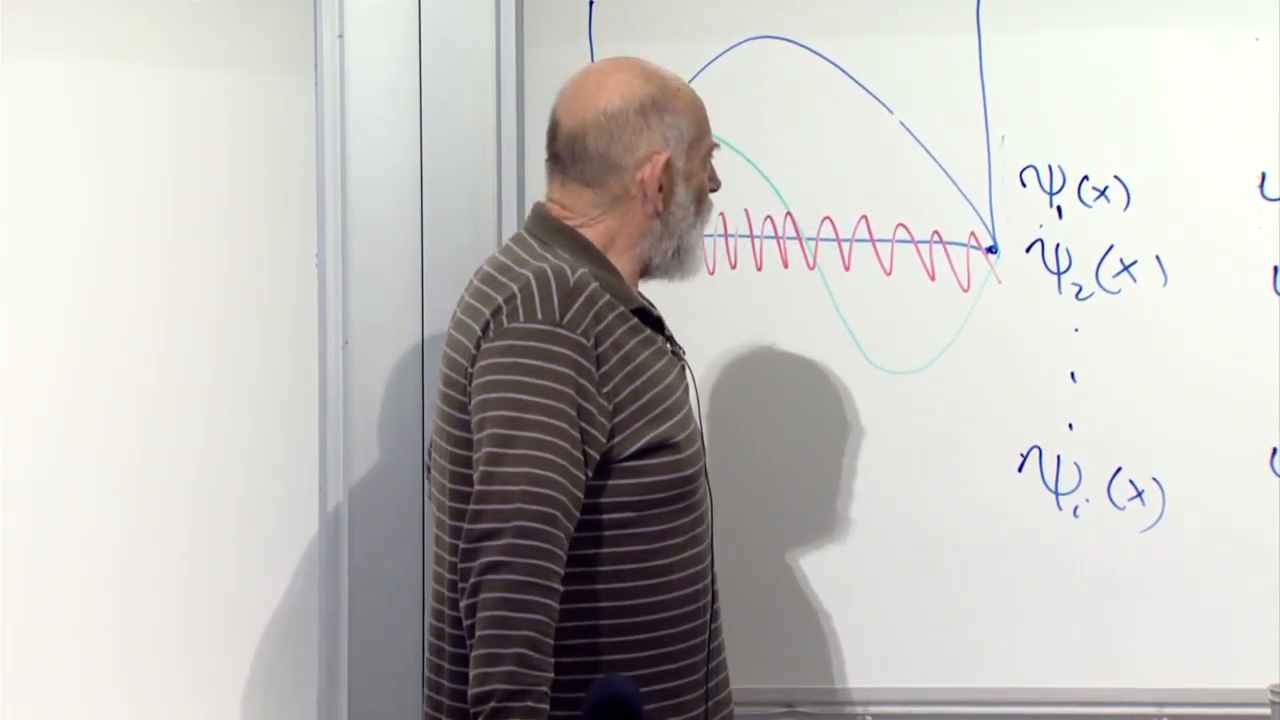
\includegraphics[width=0.9\linewidth]{lecture_06_frame_03.png}
\caption{Modos de una partícula en una caja, ordenados por energía creciente. El primer modo no tiene nodos interiores; el segundo tiene uno, y los modos superiores omitidos oscilan cada vez más rápidamente.}
\lectureframe{00:43:10}
\end{figure}

La misma estructura se puede dibujar de nuevo, sin que la oculte la pizarra en directo:
\begin{figure}[htbp]
\centering
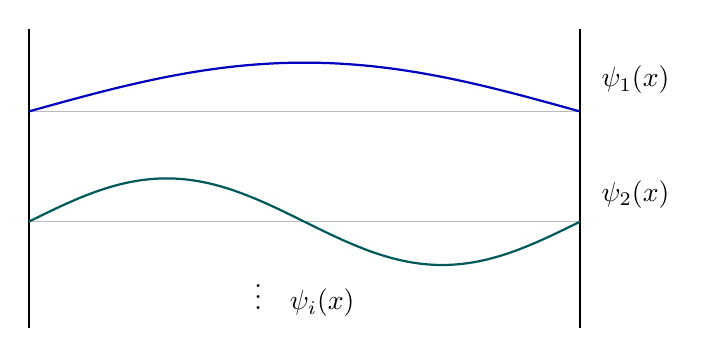
\begin{tikzpicture}[x=1cm,y=1cm]
  \draw[thick] (0,0) -- (0,3.8);
  \draw[thick] (7,0) -- (7,3.8);
  \draw[gray!55] (0,2.75) -- (7,2.75);
  \draw[gray!55] (0,1.35) -- (7,1.35);
  \draw[blue!75!black,thick,domain=0:7,samples=120]
    plot (\x,{2.75+0.62*sin(180*\x/7)});
  \draw[teal!70!black,thick,domain=0:7,samples=120]
    plot (\x,{1.35+0.55*sin(360*\x/7)});
  \node[right] at (7.15,3.15) {$\psi_1(x)$};
  \node[right] at (7.15,1.70) {$\psi_2(x)$};
  \node at (3.5,0.45) {$\vdots\quad \psi_i(x)$};
\end{tikzpicture}
\caption{Reconstrucción limpia del esquema cualitativo de los modos de la caja. El desplazamiento vertical separa las funciones propias para facilitar su lectura; no representa una coordenada física adicional.}
\end{figure}

El índice \(i\) etiqueta un estado de una partícula, no una partícula ni el número de nodos. Para la base de la caja, resulta que \(i\) es uno más que el número de nodos interiores. Cada estado tiene una energía \(\varepsilon_i\). Siguiendo la notación de la lección, podemos escribir esta energía como \(\hbar\omega_i\) o, simplemente, como \(\omega_i\) si fijamos \(\hbar=1\).

\begin{classroomqa}
\lecturetimestamp{00:39:01}
\audiencequestion{¿Era exacta la hipótesis de independencia anterior, y podría el índice \(i\) etiquetar los estados posibles de un electrón en un átomo?}
\lecturerresponse{En la construcción de modos independientes, la conmutación entre modos distintos es exacta. El índice puede etiquetar estados atómicos de una partícula. Sin embargo, si las partículas interactúan, el Hamiltoniano sencillo de modos independientes deja de describir toda la situación.}
\end{classroomqa}

\begin{classroomqa}
\lecturetimestamp{00:40:34}
\audiencequestion{¿Es bosón la partícula de la caja?}
\lecturerresponse{Podría serlo, pero, con una sola partícula, la estadística no importa. La exclusión y el intercambio solo tienen sentido cuando hay más de una partícula idéntica.}
\end{classroomqa}

\section{De los modos de la caja al espacio de Fock}

Permitamos ahora que cualquier número de bosones idénticos ocupe la caja. Un cierto número \(n_1\) puede ocupar \(\psi_1\), otro número \(n_2\) puede ocupar \(\psi_2\), y así sucesivamente. Por tanto, un estado de la base es
\begin{equation}
|n_1,n_2,n_3,\ldots\rangle.
\end{equation}
Esta es exactamente la notación que ya usamos para muchos osciladores. La identidad es estructural: asociamos un oscilador a cada estado de una partícula e identificamos el número de excitaciones del oscilador con el número de partículas que ocupan ese estado.

Los bosones son esenciales aquí porque cada \(n_i\) puede ser cualquier entero no negativo. En el caso de los fermiones, cada estado de una partícula puede estar vacío u ocupado por una sola partícula, pero nunca ocupado por dos; por eso, el álgebra ordinaria del oscilador no se puede usar sin cambios.

Ahora podemos definir los operadores mediante su acción sobre la base de números de ocupación. El operador \(a_i^\dagger\) crea una partícula en el estado de una partícula \(i\); \(a_i\) elimina una:
\begin{align}
a_i^\dagger|n_1,\ldots,n_i,\ldots\rangle
&=\sqrt{n_i+1}\,|n_1,\ldots,n_i+1,\ldots\rangle, \\
a_i|n_1,\ldots,n_i,\ldots\rangle
&=\sqrt{n_i}\,|n_1,\ldots,n_i-1,\ldots\rangle.
\end{align}
Esto no es una analogía añadida a posteriori. Es la definición de los operadores bosónicos de creación y aniquilación en esta base. Como la base genera el espacio, la definición determina por linealidad su acción sobre cualquier estado.

\begin{classroomqa}
\lecturetimestamp{00:47:11}
\audiencequestion{¿Son \(n_1,n_2,n_3\) los estados cuánticos?}
\lecturerresponse{Las etiquetas \(1,2,3,\ldots\) identifican los estados de una partícula. Los símbolos \(n_1,n_2,n_3,\ldots\) son los números de partículas que ocupan esos estados. La principal dificultad de la notación consiste en mantener separados la etiqueta del estado y su número de ocupación.}
\end{classroomqa}

\subsection{Qué hace la raíz cuadrada}

El factor \(\sqrt{n_i+1}\) no representa una partícula adicional ni un proceso físico aparte. Da al operador la normalización y el álgebra correctas. Para un modo,
\begin{align}
a a^\dagger|n\rangle
&=a\bigl(\sqrt{n+1}\,|n+1\rangle\bigr) \\
&=(n+1)|n\rangle,
\end{align}
mientras que
\begin{equation}
a^\dagger a|n\rangle=n|n\rangle.
\end{equation}
Por tanto, su diferencia es \(|n\rangle\), como exige \([a,a^\dagger]=1\). A grandes rasgos, cada uno de los dos operadores de escalera es del orden de \(\sqrt n\), pues su producto da el operador número, que es del orden de \(n\).

\begin{classroomqa}
\lecturetimestamp{00:47:52}
\audiencequestion{¿Qué significado físico concreto tiene el factor de raíz cuadrada?}
\lecturerresponse{Su función principal es la normalización matemática. Garantiza que los estados de ocupación estén normalizados, que \(a^\dagger a\) tenga el valor propio \(n\) y que los operadores de escalera satisfagan el conmutador del oscilador. A veces, la matemática misma es el significado que hace falta.}
\end{classroomqa}

\begin{classroomqa}
\lecturetimestamp{00:52:25}
\audiencequestion{¿Se han definido los operadores de creación y aniquilación solo mediante sus propiedades y su acción sobre la base?}
\lecturerresponse{Sí. Las definiciones no tienen por qué partir de una imagen más fundamental. Su valor se comprueba por sus consecuencias. Definir la acción sobre una base completa define los operadores en todas partes, y estas definiciones reproducen las relaciones de conmutación deseadas.}
\end{classroomqa}

\begin{classroomqa}
\lecturetimestamp{00:53:22}
\audiencequestion{¿Por qué \(a_i\) hace desaparecer una partícula en vez de limitarse a trasladarla a otro estado?}
\lecturerresponse{Porque \(a_i\) está definido para disminuir la ocupación del estado \(i\). La pregunta útil no es por qué una definición es verdadera, sino por qué es útil. Lo es porque la emisión y la absorción requieren operadores que cambien el número de partículas: se crea un fotón cuando se emite radiación y se aniquila cuando se absorbe.}
\end{classroomqa}

El espacio generado por todos los estados de números de ocupación es el \emph{espacio de Fock}. Contiene el vacío, todos los estados de una partícula, todos los estados de dos partículas, y así sucesivamente, sin un límite superior fijo:
\begin{equation}
\mathcal F=\mathcal H_0\oplus\mathcal H_1\oplus\mathcal H_2\oplus\cdots.
\label{eq:l06-fock-space}
\end{equation}
La notación de suma directa hace explícito lo que no mostraba la función de onda ordinaria de \(N\) partículas: todos los sectores de número de partículas pertenecen a un mismo espacio de estados.

\begin{classroomqa}
\lecturetimestamp{00:54:56}
\audiencequestion{¿Definir los operadores sobre los vectores propios de números de ocupación determina su acción sobre vectores arbitrarios? ¿Se deducen entonces los conmutadores del oscilador?}
\lecturerresponse{Exactamente. Los vectores de ocupación forman una base, así que la linealidad extiende la definición a todo el espacio de Fock. La acción sobre esa base verifica las relaciones de conmutación bosónicas. Cada estado de una partícula está representado por un oscilador, y la ocupación de ese oscilador es el número de partículas en ese estado.}
\end{classroomqa}

\subsection{El vacío y el Hamiltoniano libre}

El vacío de Fock es el estado en el que no hay partículas en ningún estado de una partícula:
\begin{equation}
|0\rangle=|0,0,0,\ldots\rangle,
\qquad a_i|0\rangle=0.
\end{equation}
La expresión \emph{estado fundamental} puede inducir a error aquí. El estado \emph{de una partícula} de menor energía es el modo \(i=1\); en el vacío de Fock no hay ninguna partícula, ni siquiera en ese modo. Si una partícula ocupa el modo más bajo, \(a_1\) puede eliminarla y devolver el sistema al vacío.

\begin{classroomqa}
\lecturetimestamp{00:56:19}
\audiencequestion{¿Qué es el vacío en términos de números de ocupación? ¿Está ocupado el estado de una partícula de menor energía?}
\lecturerresponse{En el vacío todos los números de ocupación son cero y todos los \(a_i\) lo aniquilan. El modo de una partícula de menor energía está desocupado en el vacío. Si estuviera ocupado, su operador de aniquilación podría eliminar esa partícula.}
\end{classroomqa}

Para partículas que no interactúan, la energía total es aditiva. Si una partícula en el estado \(i\) tiene energía \(\hbar\omega_i\), entonces
\begin{align}
H
&=\sum_i \hbar\omega_i N_i \\
&=\sum_i \hbar\omega_i a_i^\dagger a_i.
\label{eq:l06-free-fock-hamiltonian}
\end{align}
Hay dos interpretaciones equivalentes. Es la suma de las energías de los osciladores, uno por cada estado de una partícula. También es la suma de las energías de una partícula, cada una multiplicada por el número de partículas que tienen esa energía.

En la notación de la teoría de campos, \(a_i^\dagger\) suele llamarse operador de creación y \(a_i\), operador de aniquilación. Las notaciones más antiguas \(a_+\) y \(a_-\) expresan lo mismo.

\section{Aclaraciones antes de introducir el campo}

Varias preguntas después de la pausa permiten distinguir este nuevo recuento mediante osciladores de una partícula ordinaria que se mueve en un potencial de oscilador.

\begin{classroomqa}
\lecturetimestamp{01:06:09}
\audiencequestion{Los niveles de energía de una partícula en una caja no están igualmente espaciados. Entonces, ¿dónde está el oscilador armónico?}
\lecturerresponse{Las energías de una partícula \(\omega_i\) no tienen por qué estar igualmente espaciadas. Sin embargo, para cada modo fijo \(i\), las energías de cero, una, dos y tres partículas que no interactúan en ese modo son \(0,\omega_i,2\omega_i,3\omega_i\). Esa escalera de ocupación es el oscilador. No debe confundirse con poner una partícula en un potencial de oscilador armónico.}
\end{classroomqa}

\begin{classroomqa}
\lecturetimestamp{01:08:38}
\audiencequestion{¿Está relacionada esta construcción con la descomposición de Fourier?}
\lecturerresponse{Está profundamente relacionada. Si la base de una partícula consta de modos de momento, las funciones de modo son senos, cosenos o exponenciales complejas, y los \(a_i\) son análogos cuánticos de los coeficientes de Fourier. Una base general no tiene por qué ser trigonométrica, pero la lógica de la expansión es la misma.}
\end{classroomqa}

\begin{classroomqa}
\lecturetimestamp{01:09:07}
\audiencequestion{¿Se asigna a todas las partículas la misma energía? ¿Se incluyen las interacciones?}
\lecturerresponse{Las partículas que ocupan el mismo estado de una partícula tienen la misma energía; las que ocupan estados distintos, por lo general, no. Por ahora, las partículas son libres: no interactúan. Las interacciones añadirían términos de energía potencial, de modo que el Hamiltoniano ya no sería únicamente la suma aditiva de la ecuación~\eqref{eq:l06-free-fock-hamiltonian}.}
\end{classroomqa}

\begin{classroomqa}
\lecturetimestamp{01:10:26}
\audiencequestion{¿Qué ocurrió con el medio cuanto de energía de punto cero de cada oscilador?}
\lecturerresponse{Es una constante aditiva del Hamiltoniano. Una constante conmuta con todos los operadores, así que no altera las ecuaciones de movimiento de Heisenberg, y las mediciones ordinarias no gravitatorias dependen de diferencias de energía. Puede importar para fines especiales, pero no afecta a la construcción que estamos desarrollando aquí.}
\end{classroomqa}

La teoría libre ya es un dispositivo de recuento de extraordinaria potencia. Permite seguir no solo muchas partículas, sino también partículas que cambian de estado, aparecen, desaparecen o existen en superposiciones con distinto número total. Los operadores son más que símbolos de recuento, porque se pueden medir combinaciones hermíticas adecuadas; aun así, el recuento es una intuición inicial útil.

\begin{classroomqa}
\lecturetimestamp{01:14:03}
\audiencequestion{¿Cuál es el origen histórico de la teoría de campos y de la teoría cuántica de campos?}
\lecturerresponse{Un breve recorrido histórico comienza con la imagen física de Faraday de los campos eléctricos y magnéticos y con las ecuaciones de Maxwell para los campos clásicos. Planck introdujo los cuantos de energía al estudiar la radiación térmica; Einstein identificó la cuantización con el propio campo electromagnético y con los cuantos de luz. Heisenberg, Pauli y, en particular, Dirac contribuyeron después a construir el marco moderno de operadores hacia finales de los 1920. La catástrofe ultravioleta y la descripción cuántica de la radiación estuvieron entre los primeros problemas decisivos. Este es un esbozo histórico, no una atribución exhaustiva de prioridades.}
\end{classroomqa}

El hilo histórico también explica por qué los osciladores vuelven una y otra vez. La radiación clásica en una cavidad se descompone en modos normales. Al cuantizar esos modos, sus números de excitación se convierten en números de fotones. Los cuantos matemáticos que ocupan los modos pasan a ser partículas físicas.

\section{El operador de campo bosónico}

Sea \(\{\psi_i(x)\}\) una base completa y ortonormal de funciones de onda de una partícula. Definamos
\begin{equation}
\boxed{\Psi(x)=\sum_i a_i\,\psi_i(x)}
\label{eq:l06-field-annihilation}
\end{equation}
y su conjugado hermítico
\begin{equation}
\boxed{\Psi^\dagger(x)=\sum_i a_i^\dagger\,\psi_i^*(x)}.
\label{eq:l06-field-creation}
\end{equation}

\begin{figure}[htbp]
\centering
\includegraphics[width=0.9\linewidth]{lecture_06_frame_04.png}
\caption{Expansiones completas en modos del campo de aniquilación y de su conjugado hermítico. Las ecuaciones~\eqref{eq:l06-field-annihilation} y \eqref{eq:l06-field-creation} conservan en la composición tipográfica la misma estructura de operadores y conjugación compleja.}
\lectureframe{01:25:15}
\end{figure}

Para cualquier posición fija \(x\), cada \(\psi_i(x)\) es un número complejo ordinario. Todo el contenido de operador reside en \(a_i\) y \(a_i^\dagger\). Al variar \(x\), obtenemos un operador distinto en cada punto del espacio. Este es el sentido preciso en que \(\Psi\) es una función con valores de operador.

Si las funciones de la base son ondas planas, las ecuaciones~\eqref{eq:l06-field-annihilation} y \eqref{eq:l06-field-creation} son expansiones de Fourier cuánticas: los coeficientes de Fourier clásicos se han convertido en operadores. En una caja, la base puede constar, en cambio, de las funciones seno de la ecuación~\eqref{eq:l06-box-basis}. Sirve cualquier base completa y ortonormal de una partícula.

Ni \(\Psi\) ni \(\Psi^\dagger\) es hermítico. Se pueden construir campos observables a partir de combinaciones hermíticas como
\begin{equation}
\Psi(x)+\Psi^\dagger(x),
\qquad
i\bigl(\Psi^\dagger(x)-\Psi(x)\bigr),
\end{equation}
y más adelante se construirán densidades observables a partir de productos como \(\Psi^\dagger(x)\Psi(x)\). La tarea inmediata es entender primero qué hacen los dos campos básicos.

\begin{classroomqa}
\lecturetimestamp{01:23:14}
\audiencequestion{¿Cómo puede el miembro de la izquierda ser un operador si las funciones de modo de la derecha son funciones de onda ordinarias?}
\lecturerresponse{Las funciones \(\psi_i(x)\) son números una vez elegido \(x\). Los factores \(a_i\) son operadores. El producto de un número y un operador sigue siendo un operador, así que la suma también lo es. Al variar \(x\) se obtiene la familia completa de operadores.}
\end{classroomqa}

\section{Qué hace el campo}

El campo de aniquilación aniquila el vacío de inmediato:
\begin{equation}
\Psi(x)|0\rangle
=\sum_i\psi_i(x)a_i|0\rangle
=0.
\label{eq:l06-field-kills-vacuum}
\end{equation}
El campo de creación hace algo mucho más revelador.

Sea \(|i\rangle\) el estado de una partícula cuya función de onda es
\begin{equation}
\langle x|i\rangle=\psi_i(x).
\end{equation}
La completitud de la base de una partícula da
\begin{equation}
\sum_i|i\rangle\langle i|=1.
\label{eq:l06-completeness}
\end{equation}
Apliquemos esta identidad a un autoestado de posición:
\begin{align}
|x\rangle
&=\sum_i|i\rangle\langle i|x\rangle \\
&=\sum_i\psi_i^*(x)|i\rangle.
\label{eq:l06-position-expansion}
\end{align}
En el lenguaje de Fock, un estado de modo de una partícula es
\begin{equation}
|i\rangle=a_i^\dagger|0\rangle.
\end{equation}
Al sustituirlo en la ecuación~\eqref{eq:l06-position-expansion},
\begin{align}
|x\rangle
&=\sum_i\psi_i^*(x)a_i^\dagger|0\rangle \\
&=\Psi^\dagger(x)|0\rangle.
\label{eq:l06-local-creation}
\end{align}
Así, \(\Psi^\dagger(x)\) crea una partícula localizada en \(x\), mientras que \(\Psi(x)\) elimina allí una partícula. Un autoestado de posición está localizado mediante una delta de Dirac y es un estado generalizado no normalizable; para obtener una partícula localizada física, se integra el campo contra un paquete de ondas normalizable.\editorialnote{La lección emplea el lenguaje ideal de los autoestados de posición. La salvedad sobre el paquete de ondas recoge el significado matemático estándar sin cambiar el argumento.}

\begin{classroomqa}
\lecturetimestamp{01:36:26}
\audiencequestion{¿Qué información especifica qué tipo de partícula se crea? ¿Está el estado en \(x\) localizado mediante una delta de Dirac?}
\lecturerresponse{Se asigna un campo distinto a cada especie de partícula, así que la identidad de la partícula viene determinada por el campo que se use. El argumento \(x\) especifica dónde se crea. En la base ideal de posición, el estado creado tiene localización delta de Dirac.}
\end{classroomqa}

Entre las especies bosónicas se cuentan los fotones, los gravitones, los bosones de Higgs y los gluones, aunque los campos realistas también llevan índices internos. Incluso los fotones requieren etiquetas de polarización. La notación simplificada de campo escalar omite esas etiquetas adicionales para que el principio de creación siga siendo visible.

\subsection{El vacío no es el vector cero}

La ecuación
\begin{equation}
\Psi(x)|0\rangle=0
\end{equation}
contiene dos objetos muy distintos que se denotan con cero. El ket \(|0\rangle\) es el vacío: un estado físico normalizado que satisface
\begin{equation}
\langle0|0\rangle=1.
\end{equation}
El resultado de la derecha es el vector cero. Su norma es cero; no se puede normalizar y no representa un estado físico.

La diferencia se hace patente al sumar. Sumar el vector cero a un estado de una partícula no cambia nada. Sumar el vacío a un estado de una partícula produce una superposición genuina de sectores con distinto número de partículas. Con coeficientes normalizados,
\begin{equation}
|\chi\rangle=\frac{1}{\sqrt2}\bigl(|0\rangle+|1\rangle\bigr)
\end{equation}
asigna probabilidades iguales a cero y una partícula. No es lo mismo que \(|1\rangle\).

\begin{classroomqa}
\lecturetimestamp{01:37:23}
\audiencequestion{Si no hay ninguna partícula en \(x\), ¿\(\Psi(x)\) simplemente no hace nada? ¿Qué significa que el resultado sea cero?}
\lecturerresponse{No devuelve el estado original. Devuelve el vector nulo. El vacío es un estado normalizado que describe el espacio vacío; el vector nulo tiene longitud cero y no describe ningún estado físico. Cualquier operador que actúe sobre el vector nulo devuelve el vector nulo.}
\end{classroomqa}

\begin{classroomqa}
\lecturetimestamp{01:39:00}
\audiencequestion{¿Qué ocurre si se suma el vacío, en lugar del vector nulo, a un estado de una partícula?}
\lecturerresponse{Se obtiene una superposición con amplitudes correspondientes a distintos números de partículas. En cambio, sumar el vector nulo deja intacto el estado de una partícula. El símbolo \(|0\rangle\) designa la ocupación nula; no significa vector nulo.}
\end{classroomqa}

\begin{classroomqa}
\lecturetimestamp{01:41:56}
\audiencequestion{¿Importa el orden de una función modal y su operador de creación o aniquilación en la expansión del campo? ¿Las funciones modales son complejas?}
\lecturerresponse{La función modal es un número ordinario y, por tanto, conmuta con todos los operadores, así que el orden no importa. En general, las funciones modales pueden ser complejas; que una base elegida sea real o compleja depende del problema de una partícula de Schr\"odinger Schrödinger.}
\end{classroomqa}

\subsection{Dos partículas y la aparición de la simetría bosónica}

Para crear una partícula en \(x\) y otra en \(y\), se actúa dos veces:
\begin{equation}
|x,y\rangle
=\Psi^\dagger(y)\Psi^\dagger(x)|0\rangle.
\label{eq:l06-two-particle-state}
\end{equation}
Los puntos pueden coincidir o ser distintos. Como los operadores de creación subyacentes conmutan,
\begin{align}
[\Psi^\dagger(x),\Psi^\dagger(y)]
&=\sum_{i,j}\psi_i^*(x)\psi_j^*(y)
[a_i^\dagger,a_j^\dagger] \\
&=0.
\end{align}
Se sigue que
\begin{equation}
\Psi^\dagger(y)\Psi^\dagger(x)|0\rangle
=\Psi^\dagger(x)\Psi^\dagger(y)|0\rangle.
\label{eq:l06-boson-exchange}
\end{equation}
Intercambiar el orden de las dos partículas no cambia nada. Esta es precisamente la simetría de intercambio bosónica. Por tanto, podríamos haber partido del álgebra del oscilador y \emph{deducido} que las partículas construidas con operadores de creación que conmutan son bosones. Para los fermiones se necesitarán, en cambio, operadores que anticonmuten.

\begin{classroomqa}
\lecturetimestamp{01:42:37}
\audiencequestion{¿Cómo se añade una segunda partícula al estado de una partícula?}
\lecturerresponse{Se aplica otro campo de creación. Para añadirla en \(y\), se actúa con \(\Psi^\dagger(y)\) a la izquierda de \(\Psi^\dagger(x)\). El resultado es el estado de dos partículas de la ecuación~\eqref{eq:l06-two-particle-state}.}
\end{classroomqa}

\begin{classroomqa}
\lecturetimestamp{01:46:04}
\audiencequestion{¿La conmutatividad de los dos campos de creación equivale plenamente a simetrizar el estado de dos partículas?}
\lecturerresponse{Sí. Hace que el estado con una partícula en \(x\) y otra en \(y\) sea idéntico al estado que se obtiene al intercambiar las etiquetas. Esta es la propiedad de intercambio que define a los bosones idénticos.}
\end{classroomqa}

\begin{classroomqa}
\lecturetimestamp{01:46:32}
\audiencequestion{¿Significa esto que las partículas en \(x\) y \(y\) deben ser bosones del mismo tipo?}
\lecturerresponse{Sí. Los argumentos \(x\) y \(y\) son posiciones, mientras que un campo describe una especie. Las distintas especies y las etiquetas adicionales, como las dos polarizaciones del fotón, requieren componentes de campo diferentes.}
\end{classroomqa}

\section{Por qué importa que el número de partículas pueda variar}

Si un problema contuviera exactamente 37 partículas para siempre, el lenguaje de campos sería una herramienta opcional de contabilidad. Su verdadera utilidad aparece cuando las partículas pueden emitirse y absorberse, y sobre todo cuando el propio número de partículas es una variable cuántica. El espacio de Fock permite estados de la forma
\begin{equation}
|\Phi\rangle
=c_0|0\rangle+c_1|1\rangle+c_2|2\rangle+\cdots,
\qquad
\sum_{n=0}^{\infty}|c_n|^2=1.
\end{equation}
Un campo láser es un ejemplo importante: en general, no es un estado con un número de fotones definido, sino una superposición de muchos sectores de número.

El vínculo entre partículas y campos ya es explícito. Los operadores modales cuentan partículas y modifican su número en los estados propios de la energía; el campo combina esos operadores con un conjunto completo de funciones de onda para que se puedan crear o eliminar partículas en posiciones determinadas. El álgebra de los osciladores armónicos se ha convertido en el lenguaje elemental de un campo cuántico bosónico.
